%Template and commentary by Michael Rouleau: https://github.com/mikerouleau/ME4842.git
%Text primarily from Dr. Stutts' Systems Laboratory Manual /ref{Stutts}
%Last Updated: Feb 15, 2019

%----This template includes equation captions and numbering BELOW the equation----%

\documentclass[11pt,letter]{report}
\usepackage[margin=1in]{geometry} %make margins 1"
\usepackage[justification=centering, format=plain,
font=it, margin=1in]{caption} %all captions centered and made italics by default
\usepackage{amsmath, amssymb} %advanced math extensions
\usepackage{graphicx} %enhanced graphics handling/management
\usepackage{float} %create floating containers
\usepackage{aliascnt} %alias counters as needed

%make equations floating objects and alias counter - needed for formatting requirements
\newaliascnt{eqfloat}{equation} %make the counter alias eqfloat
\newfloat{eqfloat}{!htb}{eqflts} %make the float container for equations
\floatname{eqfloat}{Equation} %change name so captions read "Equation" X:
        
%nontraditional usage of author to meet formatting requirements
\title{\Huge{A Systems Lab Memo}}
\author{Section \#, Group \#: \\
  Group Member 1 \quad Group Member 2 \quad Group Member 3 \quad Group Member 4 \\ GTA: Blaine Allen \\\\ Prepared By: \\ Michael Rouleau\thanks{Nearly all of this information is from the course manual\cite{Stutts}; I simply formatted it.}}
\date{\today}

\begin{document}
\maketitle

\section*{Abstract}
The Abstract should be approximately 100-150 words in length. This may be a very strict limit in some cases. For ME4842, the limit will be somewhat flexible. This should include what the objective of the experiment was and its importance, any theory the experiment is based on, major findings and trends found in your results, and a brief summary of your interpretations and conclusions. You should not reference anything in the abstract; this section should be completely independent from the rest of the report.

\section*{Procedure}
Here, you will briefly explain what steps you followed in conducting the experiment. The procedure should state what is not covered in the lab manual and what decisions you made in order to accomplish the experiment. It may be handy to organize this section as a list.

\section*{Results}
Here, you will explain the data you took, and any calculations that you made. This section should be the longest in the report. Many results can be displayed using objects similar to Table~\ref{table:Civil Cheese} and Figure~\ref{fig:Cat Lord}, displayed below.

%Tools such as those at https://www.tablesgenerator.com/ may be useful for creating tables quickly.

%example table formatting
\begin{table}[!htb]
\caption{ Annual Per Capita Consumption of Mozzarella Cheese and Civil Engineering Doctorates Awarded \cite{Vigen}}%\cite{name} refers to a specific bibliography entry.
\label{table:Civil Cheese} %use this label to refer to the object elsewhere, as shown in the previous paragraph.
\centering
	\begin{tabular}{|c|c|c|}
	\hline
	\textbf{Year} & 
	\textbf{\begin{tabular}[c]{@{}c@{}}
			Civil Engineering\\ 
			Doctorates\end{tabular}} &
	\textbf{\begin{tabular}[c]{@{}c@{}}
			Mozzarella\\
			Cheese Consumption
	\end{tabular}} \\ \hline

2000  & 480  & 9.3     \\ \hline
2001  & 501  & 9.7     \\ \hline
2002  & 540  & 9.7     \\ \hline
2003  & 552  & 9.7     \\ \hline
2004  & 547  & 9.9     \\ \hline
2005  & 622  & 10.2    \\ \hline
2006  & 655  & 10.5    \\ \hline
2007  & 701  & 11.0    \\ \hline
2008  & 712  & 10.6    \\ \hline
2009  & 708  & 10.6    \\ \hline
\end{tabular}
\end{table}

%example figure formatting
\begin{figure}[!htb]
\label{fig:Cat Lord}
\centering
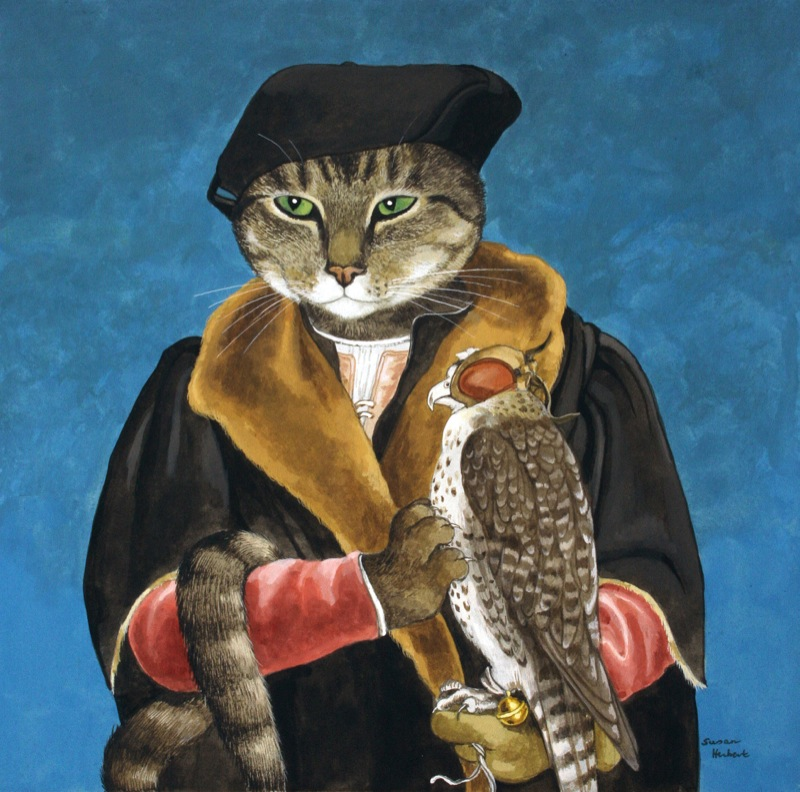
\includegraphics[scale=0.4]{cat-painting}%include full file path unless source file is in the same directory.
\caption{Robert Cheseman (Holbein)\cite{Herbert}}
\end{figure}

\begin{enumerate} %start numbered list
  \item You should be mindful of the number of significant digits you use in your results.
  \item Use consistent units and suitable unit prefixes.
  \item When referring to equations, figures, tables, and appendices in your memo you must always capitalize E in equation F in figure, T in table, and A in appendix.
  \item To reference an equation from the manual don't say "according to Equation 8.25 in the manual". The correct way to do this is: "according to Equation 2 [X]”. Note Equation 2 is an equation in your memo and has its own number and [X] is the citation number in your reference section corresponding to the appropriate source.
  \item Table, figure, and equation titles: Tables get titles on top. Figures and equations get the title on the bottom.
  \item Tables, figures and equations must be part of the written text. That is you should put your table, figure, and equation right below the paragraph where they are first mentioned.
  \item Only include necessary data in tables that are related to the analysis of the experiment.
\end{enumerate}

\section*{Discussion Questions}
In this section, simply answer each question from the lab manual in order. It may be wise to number your responses. Some responses require equations. Equation~\ref{Quadratic} displays the proper formatting; Equation~\ref{eq:Dirac} is a more complex example.

\begin{eqfloat}[!htb]
\begin{equation*}
x=\frac{-b\pm\sqrt{b^2-4ac}}{2a}
\end{equation*}
\caption{The Quadratic Formula}\label{Quadratic}
\end{eqfloat}
	
\begin{eqfloat}
\begin{equation*}
\left (
    \beta mc^2 + c 
       \left ( 
           \sum_{n=1}^3 \alpha_n p_n 
       \right )
\right )
\psi(x,t)
=
i \hbar \dfrac{\partial \psi(x,t) }{\partial t}
\end{equation*}
\caption{The Original Dirac Equation}\label{eq:Dirac}
\end{eqfloat}
%note that the equation numbering auto-increments and the in-line references update accordingly. Tables and figures behave the same way.

\section*{Conclusion}
Conclusions should clearly state how well the objective was met, any errors that were part of your data collections or would have affected results, suggestions to improve experimental data collection, and what you might have done better. If you are going to make suggestions for improving the experiment, ensure they are technically sound and would make a significant impact on results.

%A pure LaTeX bibliography 
\begin{thebibliography}{3} %{3} is the number of entries to be added. The maximum value is 99.

\bibitem{Herbert}
  Herbert, S.,\emph{Robert Cheseman (Holbein).}
  Chris Beetles Gallery, London, England, www.chrisbeetles.com/gallery/animals/cats/robert-cheseman-holbein.html. Accessed 8 Nov. 2018.
  
\bibitem{Stutts}
  Stutts, D.S., \emph{Mechanical Engineering Systems Laboratory Manual.}
  Department of Mechanical and Aerospace Engineering, Missouri University of Science and Technology, 3 Oct. 2018. 130-131.
  
\bibitem{Vigen}
  Vigen, T., \emph{15 Insane Things That Correlate With Each Other.}
  Spurious Correlations, tylervigen.com/spurious-correlations. Accessed 8 Nov. 2018.

\end{thebibliography}

\newpage %force a new page
\section*{Appendix A: Additional Data}
Only thing to put in the appendix is programming codes, program code output, and large raw data tables that are not referenced in any results.

\end{document}